\documentclass[a4paper, 11pt, notitlepage, english]{article}

\usepackage{babel}
\usepackage[utf8]{inputenc}
\usepackage[T1]{fontenc, url}
\usepackage{textcomp}
\usepackage{amsmath, amssymb}
\usepackage{amsbsy, amsfonts}
\usepackage{graphicx, color}
\usepackage{parskip}
\usepackage{framed}
\usepackage{amsmath}
\usepackage{xcolor}
\usepackage{multicol}
\usepackage{url}
\usepackage{flafter}
\usepackage{simplewick}
\usepackage{amsthm}
\usepackage{bbold}



\newtheorem{theorem}[]{Wick's Theorem}[]

\DeclareUnicodeCharacter{00A0}{~}

\usepackage{geometry}
\geometry{headheight=0.01mm}
\geometry{top=20mm, bottom=20mm, left=34mm, right=34mm}

\renewcommand{\arraystretch}{2}
\setlength{\tabcolsep}{10pt}
\makeatletter
\renewcommand*\env@matrix[1][*\c@MaxMatrixCols c]{%
  \hskip -\arraycolsep
  \let\@ifnextchar\new@ifnextchar
  \array{#1}}
%
% Parametere for inkludering av kode fra fil
%
\usepackage{listings}
\lstset{language=python}
\lstset{basicstyle=\ttfamily\small}
\lstset{frame=single}
\lstset{keywordstyle=\color{red}\bfseries}
\lstset{commentstyle=\itshape\color{blue}}
\lstset{showspaces=false}
\lstset{showstringspaces=false}
\lstset{showtabs=false}
\lstset{breaklines}

%
% Definering av egne kommandoer og miljøer
%
\newcommand{\dd}[1]{\ \text{d}#1}
\newcommand{\f}[2]{\frac{#1}{#2}} 
\newcommand{\beq}{\begin{equation}}
\newcommand{\eeq}{\end{equation}}
\newcommand{\bra}[1]{\langle #1|}
\newcommand{\ket}[1]{|#1 \rangle}
\newcommand{\braket}[2]{\langle #1 | #2 \rangle}
\newcommand{\braup}[1]{\langle #1 \left|\uparrow\rangle\right.}
\newcommand{\bradown}[1]{\langle #1 \left|\downarrow\rangle\right.}
\newcommand{\av}[1]{\left| #1 \right|}
\newcommand{\op}[1]{\hat{#1}}
\newcommand{\braopket}[3]{\langle #1 | {#2} | #3 \rangle}
\newcommand{\ketbra}[2]{\ket{#1}\bra{#2}}
\newcommand{\pp}[1]{\frac{\partial}{\partial #1}}
\newcommand{\ppn}[1]{\frac{\partial^2}{\partial #1^2}}
\newcommand{\up}{\left|\uparrow\rangle\right.}
\newcommand{\upup}{\left|\uparrow\uparrow\rangle\right.}
\newcommand{\down}{\left|\downarrow\rangle\right.}
\newcommand{\downdown}{\left|\downarrow\downarrow\rangle\right.}
\newcommand{\updown}{\left|\uparrow\downarrow\rangle\right.}
\newcommand{\downup}{\left|\downarrow\uparrow\rangle\right.}
\newcommand{\bupup}{\left.\langle\uparrow\uparrow\right|}
\newcommand{\bdowndown}{\left.\langle\downarrow\downarrow\right|}
\newcommand{\bupdown}{\left.\langle\uparrow\downarrow\right|}
\newcommand{\bdownup}{\left.\langle\downarrow\uparrow\right|}
\renewcommand{\d}{{\rm d}}
\newcommand{\Res}[2]{{\rm Res}(#1;#2)}
\newcommand{\To}{\quad\Rightarrow\quad}
\newcommand{\eps}{\epsilon}
\newcommand{\inner}[2]{\langle #1 , #2 \rangle}
\renewcommand{\u}{\uparrow}
\renewcommand{\d}{\downarrow}
\newcommand{\dddd}{\d\d\d\d}
\newcommand{\uddd}{\u\d\d\d}
\newcommand{\dudd}{\d\u\d\d}
\newcommand{\ddud}{\d\d\u\d}
\newcommand{\dddu}{\d\d\d\u}
\newcommand{\uudd}{\u\u\d\d}
\newcommand{\udud}{\u\d\u\d}
\newcommand{\uddu}{\u\d\d\u}
\newcommand{\duud}{\d\u\u\d}
\newcommand{\dudu}{\d\u\d\u}
\newcommand{\dduu}{\d\d\u\u}
\newcommand{\uuud}{\u\u\u\d}
\newcommand{\uudu}{\u\u\d\u}
\newcommand{\uduu}{\u\d\u\u}
\newcommand{\duuu}{\d\u\u\u}
\newcommand{\uuuu}{\u\u\u\u}
\newcommand{\m}{\text{-}}




\newcommand{\bt}[1]{\boldsymbol{#1}}
\newcommand{\mat}[1]{\textsf{\textbf{#1}}}
\newcommand{\I}{\boldsymbol{\mathcal{I}}}
\newcommand{\p}{\partial}
%
% Navn og tittel
%
\author{Jonas van den Brink \\ \texttt{j.v.brink@fys.uio.no}}
\title{Problem set 5 \\ FYS-KJM4480}

\begin{document}
\maketitle

This week, we start using diagrams to elucidate our second quantization notation. We now represent states relative to the Fermi vacuum by using simple diagrams following certain schematical rules. Let us show some examples before we turn to the exercises.

\section*{Exercise 9}
\subsection*{a)}

We are looking at the three following diagrams
\begin{figure}[h!]
	\centering
	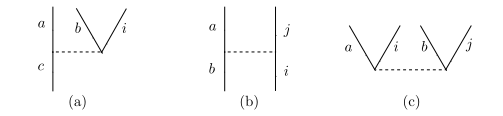
\includegraphics[width=\textwidth]{exercise9a}
\end{figure}

All three diagrams represent operators, and in this case they are operators corresponding to some sort of two-body interaction.

For diagram \textbf{(a)}, we see that below the interaction there is a single particle line, as the line is pointed upwards. Above the interaction, there are two particle lines and a single hole line, i.e., two lines pointing upwards and one pointed downwards. We thus see that this operator has an excitation level of $+1$, as it creates a new particle-hole pair. The interaction also has a matrix element associated with it as a multiplicative factor. Writing out the operator associated with the diagram algebraicly, we have 
$$\sum_{abci} \braopket{ab}{\op{v}}{ci}\{\op{a}^\dagger\op{b}^\dagger\op{i}\op{c}\}.$$

For diagram \textbf{(b)}, we see that there is a single particle line and single hole line both above and below the interaction, i.e., this diagram has an excitation level of 0 (no particle-hole pairs are created or destroyed). Algebraicly the operator can be written as
$$-\sum_{abij}\braopket{ai}{\op{v}}{bj}\{\op{a}^\dagger\op{i}^\dagger\op{j}\op{b}\}.$$

For diagram \textbf{(c)}, we see that there are no lines below the interaction, and four lines above it, two particle lines and two hole lines. This means that the interaction creates two particle-hole pairs and has an excitation level of $+2$. We can write out this operator as
$$\sum_{abij}\braopket{ab}{\op{v}}{ij}\{\op{a}^\dagger\op{b}^\dagger\op{j}\op{i}\}.$$
As there are no lines below the interaction, this is the only operator of the three which can act on the Fermi vaccuum and produce a non-trivial result, as it is the only diagram that has nothing below the interaction.

\subsection*{b)}
Last week, we found that a general two-body operator could be written
$$\op{H}_I = \frac{1}{4}\sum_{pqrs}\braopket{pq}{\op{v}}{rs}_{\rm AS}\{\op{p}^\dagger \op{q}^\dagger\op{s}\op{r}\} + \sum_{pqi}\braopket{pi}{\op{v}}{qi}_{\rm AS}\{\op{p}^\dagger\op{q}\} + \frac{1}{2}\sum_{ij}\braopket{ij}{\op{v}}{ij}_{\rm AS}.$$
We now want to find the diagrammatic expression for $\braopket{c}{\op{H}_I}{c}$, where $\ket{c}$ denotes the core-state, which is a different name for the Fermi vacuum. 

To find the diagrammatic expression for the matrix element, we first realize that the first two terms in the operator will vanish when we take the core-expectation as the normal-products vanish. From a diagram point-of-view this becomes apparant as these forms of the interactions have free lines above and below the interaction which we cannot attach to the vaccuum states above and below. We are therefore left with the only elements where there are no free lines out of the interaction, there are two such diagrams for a general two-body operator. We then have
\begin{center}
	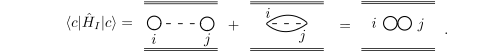
\includegraphics[width=\textwidth]{exercise9b}
\end{center}
Here the first two diagrams are Goldstone diagrams, and the final diagram is a Hugenholtz diagram. The Goldstone diagrams represent the direct and exchange sums
$$\frac{1}{2}\sum_{ij} \braopket{ij}{\op{v}}{ij} \qquad \mbox{and} \qquad -\frac{1}{2}\sum_{ij} \braopket{ji}{\op{v}}{ij},$$
respectively. The Hugenholtz diagram combine these two terms into a single, asymmetrized term.
$$\frac{1}{2}\sum_{ij} \braopket{ij}{\op{v}}{ij}_{\rm AS}.$$
In each case, the factor of 1/2 can be read out directly from the diagram. As each diagram has two equivalent hole lines.

\clearpage

\section*{Exercise 10}
We now look at a system with two distinct energy levels, each with a degeneration of $d=4$. We denote the energy levels with the quantum numbers $\sigma = \{-1,1\}$, and the four sublevels with the numbers $p=1,2,3,4$. The energy of the two levels are $\eps_1 = \eps/2$ and $\eps_2 = -\eps/2$. We define the single-particle states from the quantum numbers, $\sigma$ and $p$ and assume that these span an orthonormal basis. We then have
$$\ket{u_{p\sigma}} = \op{a}^\dagger \ket{0}.$$
We also assume the Hamiltonian of the system to be
$$\op{H} = \frac{\eps}{2}\sum_{p\sigma} \sigma \op{a}_{p\sigma}^\dagger\op{a}_{p\sigma} + \frac{V}{2}\sum_{pp'\sigma} \sigma \op{a}_{p\sigma}^\dagger \op{a}_{p\sigma'}^\dagger \op{a}_{-p\sigma'} \op{a}_{-p\sigma} +
\frac{W}{2}\sum_{pp'\sigma} \op{a}_{p\sigma}^\dagger \op{a}_{-p\sigma'}^\dagger \op{a}_{p\sigma'} \op{a}_{-p\sigma},$$
where we will refer to the first, second and third term as $\op{H}_0$, $\op{H}_1$ and $\op{H}_2$ respectively.

\subsubsection*{a)}

In this exercise, we will introduce some quasispin operators and look at the commutation relations between them. The commutator between two operators is defined as
$$[\op{A},\op{B}] = \op{A}\op{B} - \op{B}\op{A}.$$
From this definition, some properties of commutators is readily apparent
$$[\op{B},\op{A}] = \op{B}\op{A} - \op{A}\op{B} = -[\op{A},\op{B}].$$
As well as
$$[\op{A}\op{B},\op{C}] =  \op{A}\op{B}\op{C} +\underbrace{(-\op{A}\op{C}\op{B} + \op{A}\op{C}\op{B})}_{=0} - \op{C}\op{A}\op{B} = \op{A}[\op{B},\op{C}] + [\op{A},\op{C}]\op{B}.$$
In quantum mechanics, we define the angular momentum operators in the three spatial dimensions as $\op{L}_x, \op{L}_y$ and $\op{L}_z$. We know that these have commutation relations\footnote{See for example \emph{Introduction to Qunatum Mechanics} by Griffiths, sec.\ 4.3.}
$$[\op{L}_x, \op{L}_y] = i\hbar \op{L}_z, \quad [\op{L}_y, \op{L}_z] = i\hbar \op{L}_x, \quad [\op{L}_z, \op{L}_x] = i\hbar \op{L}_y.$$
We also define $\op{L}^2 = \op{L}_x^2 + \op{L}_y^2 + \op{L}_z^2$, which commutes with all three of the first operators
$$[\op{L}^2, \op{L}_x] = [\op{L}^2, \op{L}_y] = [\op{L}^2, \op{L}_z] = 0.$$
It is also normal to define the operators $\op{L}_\pm = \op{L}_x \pm i\op{L}_y$, which have the commutation relations
$$[\op{L}_+,\op{L}_-] = 2\hbar\op{L}_z, \qquad  [\op{L}_z, \op{L}_\pm] = \pm \hbar \op{L}_\pm, \qquad [\op{L}^2, \op{L}_\pm] = 0.$$
For spin, there are exactly analogous operators, which shouldn't come as a surprise, as spin is nothing more than \emph{intrinsic} angular momentum. 

We now introduce the \emph{quasispin} operators
\begin{align*}
\op{J_\pm} &= \sum_p \op{a}_{p\pm}^\dagger \op{a}_{p\mp}, \\
\op{J_z} &= \frac{1}{2}\sum_{p\sigma}\sigma a_{p\sigma}^\dagger a_{p\sigma}, \\
\op{J}^2 &= \op{J}_+\op{J}_- + \op{J}_z^2 - \op{J}_z,
\end{align*}
to our system. We will show that these have commutation relations that are similar to those of the angular momentum and spin operators.

We start with
$$[\op{J_+}, \op{J_-}] = \op{J_+}\op{J_-} - \op{J_-}\op{J_+},$$
inserting for the operators gives
$$[\op{J_+}, \op{J_-}] = \sum_{pp'}\bigg( \op{a}_{p+}^\dagger \op{a}_{p-} \op{a}_{p'-}^\dagger \op{a}_{p'+} - \op{a}_{p'-}^\dagger \op{a}_{p'+} \op{a}_{p+}^\dagger \op{a}_{p-}\bigg).$$
We now use the anti-commutation relations of the creation and annihilation operators
$$\{\op{a}_\alpha^\dagger, \op{a}_\beta^\dagger \} = \{\op{a}_\alpha, \op{a}_\beta \} = 0, \qquad \{\op{a}_\alpha^\dagger, \op{a}_\beta \} = \delta_{\alpha\beta},$$
to find
\begin{align*}
[\op{J}_+,\op{J}_-] &= \sum_{pp'}\bigg( \op{a}_{p+}^\dagger \op{a}_{p-} \op{a}_{p'-}^\dagger \op{a}_{p'+} - \op{a}_{p'-}^\dagger \big(\delta_{pp'} - \op{a}_{p+}^\dagger\op{a}_{p'+} \big) \op{a}_{p-}\bigg) \\
&= \sum_{pp'}\bigg( \op{a}_{p+}^\dagger \op{a}_{p-} \op{a}_{p'-}^\dagger \op{a}_{p'+} + \op{a}_{p+}^\dagger  \op{a}_{p'-}^\dagger  \op{a}_{p-} \op{a}_{p'+} - \delta_{pp'} \op{a}_{p'-}^\dagger\op{a}_{p-}\bigg) \\
&= \sum_{pp'}\bigg( \op{a}_{p+}^\dagger \op{a}_{p-} \op{a}_{p'-}^\dagger \op{a}_{p'+} + \op{a}_{p+}^\dagger  \big(\delta_{pp'} -\op{a}_{p-}\op{a}_{p'-}^\dagger \big) \op{a}_{p'+} - \delta_{pp'} \op{a}_{p'-}^\dagger\op{a}_{p-}\bigg) \\
&= \sum_{pp'}\bigg( \op{a}_{p+}^\dagger \op{a}_{p-} \op{a}_{p'-}^\dagger \op{a}_{p'+} - \op{a}_{p+}^\dagger \op{a}_{p-}\op{a}_{p'-}^\dagger + \delta_{pp'}\big(\op{a}_{p+}^\dagger \op{a}_{p'+} - \op{a}_{p'-}^\dagger\op{a}_{p-}\big)\bigg) \\
&= \sum_{pp'} \delta_{pp'}\big(\op{a}_{p+}^\dagger \op{a}_{p'+} - \op{a}_{p'-}^\dagger\op{a}_{p-}\big).
\end{align*}
The Kronecker-delta kills one sum, and we are left with
$$[\op{J}_+,\op{J}_-] = \sum_p \op{a}_{p+}^\dagger \op{a}_{p+} - \op{a}_{p-}^\dagger\op{a}_{p-} = \sum_{p\sigma} \sigma \op{a}_{p\sigma}^\dagger\op{a}_{p\sigma} = 2 \op{J}_z.$$
So we see that the result is equal to that for the angular momentum operators, if we set $\hbar=1$.
Next we look at $[J_z, J_+]$, writing out the operators gives
$$[J_z, J_+] = \frac{1}{2}\sum_{p p'} \big(\op{a}_{p+}^\dagger \op{a}_{p+} - \op{a}_{p-}^\dagger\op{a}_{p-}\big)\op{a}_{p'+}^\dagger \op{a}_{p'-}  - \op{a}_{p'+}^\dagger \op{a}_{p'-}\big(\op{a}_{p+}^\dagger \op{a}_{p+} - \op{a}_{p-}^\dagger\op{a}_{p-}\big).$$
Which we see gives a total of 4 terms,
\begin{align*}
[J_z, J_+] = \frac{1}{2}\sum_{p p'} \bigg(
&\op{a}_{p+}^\dagger \op{a}_{p+}\op{a}_{p'+}^\dagger \op{a}_{p'-} 
- \op{a}_{p-}^\dagger \op{a}_{p-}\op{a}_{+p'}^\dagger\op{a}_{p'-} \\
&- \op{a}_{p'+}^\dagger \op{a}_{p'-}\op{a}_{p+}^\dagger \op{a}_{p+} 
+ \op{a}_{+p'}^\dagger\op{a}_{p'-}\op{a}_{p-}^\dagger \op{a}_{p-}\bigg).
\end{align*}
We now see that we can use the anti-commutation relations to make the first and third terms mostly cancel out, and the same for the second and fourth terms:
\begin{align*}
(1) + (3) &=
\op{a}_{p+}^\dagger \op{a}_{p+}\op{a}_{p'+}^\dagger \op{a}_{p'-} 
- \op{a}_{p'+}^\dagger \op{a}_{p'-}\op{a}_{p+}^\dagger \op{a}_{p+}  \\
&= 
\op{a}_{p+}^\dagger \op{a}_{p+}\op{a}_{p'+}^\dagger \op{a}_{p'-} 
+ \op{a}_{p+}^\dagger \op{a}_{p'+}^\dagger\op{a}_{p+}\op{a}_{p'-}  \\
&=
\op{a}_{p+}^\dagger \op{a}_{p+}\op{a}_{p'+}^\dagger \op{a}_{p'-} 
+ \op{a}_{p+}^\dagger \big(\delta_{pp'}  - \op{a}_{p+}\op{a}_{p'+}^\dagger\big)\op{a}_{p'-}  \\
&= \delta_{pp'} \op{a}_{p+}^\dagger \op{a}_{p'-} 
\end{align*}
Where we only got a single surviving Kronecker-delta contribution, because the $\sigma$ quantum number was different in the other case. The second and fourth term gives
\begin{align*}
(4) + (2) &=
\op{a}_{+p'}^\dagger\op{a}_{p'-}\op{a}_{p-}^\dagger \op{a}_{p-} - \op{a}_{p-}^\dagger \op{a}_{p-}\op{a}_{+p'}^\dagger\op{a}_{p'-} \\
&=  \op{a}_{+p'}^\dagger\op{a}_{p'-}\op{a}_{p-}^\dagger \op{a}_{p-} + \op{a}_{+p'}^\dagger\op{a}_{p-}^\dagger \op{a}_{p'-} \op{a}_{p-} \\
&=  \op{a}_{+p'}^\dagger\op{a}_{p'-}\op{a}_{p-}^\dagger \op{a}_{p-} + \op{a}_{+p'}^\dagger\big( \delta_{pp'} -  \op{a}_{p'-}\op{a}_{p-}^\dagger\big) \op{a}_{p-} \\
&= \delta_{pp'}\op{a}_{+p'}^\dagger \op{a}_{p-}
\end{align*}
Combining the results, we get
\begin{align*}
[J_z, J_+] &= \frac{1}{2}\sum_{pp'} 2 \delta_{pp'}\op{a}_{+p'}^\dagger \op{a}_{p-} \\
&= \sum_{p} \op{a}_{+p'}^\dagger \op{a}_{p-} \\
&= {J}_+.
\end{align*}
Using the exact same approach, we find that
$$[\op{J_z},\op{J}_-] = -J_-.$$
Meaning we have found the commutation relation
$$[\op{J}_z,\op{J}_\pm] = \pm \op{J}_\pm.$$
Which again is similar to the angular momentum case, again with $\hbar=1$.

We now turn to $[\op{J}^2, \op{J}_z]$, we then have
\begin{align*}
[\op{J}^2, \op{J}_z] = [\op{J}_+\op{J}_-, \op{J}_z] + [\op{J}_z^2, \op{J}_z] - [\op{J}_z, \op{J}_z],
\end{align*}
The last two terms here are of course zero, as any operator commutes with itself. So we have
\begin{align*}
[\op{J}^2, \op{J}_z] &= [\op{J}_+\op{J}_-, \op{J}_z] \\
&= \op{J}_+[\op{J}_-, \op{J}_z] + [\op{J}_+, \op{J}_z]\op{J}_-,
\end{align*}
And these commutators we just found, so we can insert for them to find
\begin{align*}
[\op{J}^2, \op{J}_z] &= \op{J}_+\op{J}_- - \op{J}_+\op{J}_- = 0.
\end{align*}

Finally, we want to show that $[\op{J}^2, \op{J}_\pm]=0$, we have
\begin{align*}
[\op{J}^2, \op{J}_\pm] &= [\op{J}_+\op{J}_-, \op{J}_\pm] + [\op{J}_z^2, \op{J}_\pm] - [\op{J}_z, \op{J}_\pm] \\
&= \op{J}_+[\op{J}_-, \op{J}_\pm] + [\op{J}_+, \op{J}_\pm]\op{J}_-  + \op{J}_z[\op{J}_z, \op{J}_\pm] + [\op{J}_z, \op{J}_\pm]\op{J}_z - [\op{J}_z, \op{J}_\pm] 
\end{align*}
Let us look at the $\op{J_+}$ case first
\begin{align*}
[\op{J}^2, \op{J}_+] &= \op{J}_+[\op{J}_-, \op{J}_+] + \op{J}_z[\op{J}_z, \op{J}_+] + [\op{J}_z, \op{J}_+]\op{J}_z - [\op{J}_z, \op{J}_+] \\
&= -2\op{J}_+\op{J}_z + \op{J}_z\op{J}_+ + \op{J}_+\op{J}_z -  [\op{J}_z, \op{J}_+] \\
&= \op{J}_z\op{J}_+ - \op{J}_+\op{J}_z -  [\op{J}_z, \op{J}_+] \\
&= [\op{J}_z, \op{J}_+] -  [\op{J}_z, \op{J}_+] \\
&= 0.
\end{align*}
And unsuprisingly, the $\op{J}_-$ results in the same
\begin{align*}
[\op{J}^2, \op{J}_\pm] &= [\op{J}_+, \op{J}_-]\op{J}_-  + \op{J}_z[\op{J}_z, \op{J}_-] + [\op{J}_z, \op{J}_-]\op{J}_z - [\op{J}_z, \op{J}_-] =  [\op{J}_z, \op{J}_-] - [\op{J}_z, \op{J}_-] = 0.
\end{align*}
So we see that our quasispin operators obey the same commutation relations as the angular momentum operators
$$[\op{J}_+, \op{J}_-] = 2\op{J}_z, \qquad [\op{J}_z, \op{J}_\pm] = \pm\op{J}_\pm, \qquad [\op{J}^2, \op{J}_z] = [\op{J}^2, \op{J}_\pm] = 0.$$

\clearpage

\subsubsection*{b)}
We now want to express the Hamiltonian of our system in terms of the quasispin operators. Let us focus on each term of the Hamiltonian seperately. The first term is the easiest, we immediately recognize it as the $\op{J}_z$-operator,
$$\op{H}_0 = \frac{1}{2}\eps \sum_{p\sigma} \sigma \op{a}_{p\sigma}^\dagger \op{a}_{p\sigma} = \eps\op{J}_z.$$
In the second term we have to rearrange the creation and annihilation operators a bit, but it won't give us any Kronecker deltas, as the $\sigma$ quantum number is different for the operators we interchange 
\begin{align*}
\op{H}_1 &= 
\frac{1}{2}V\sum_{pp'\sigma} \op{a}_{p\sigma}^\dagger \op{a}_{p\sigma'}^\dagger \op{a}_{-p\sigma'} \op{a}_{-p\sigma} \\
&= \frac{1}{2}V\sum_{\sigma} \sum_p\op{a}_{p\sigma'}^\dagger \sum_{p'}\op{a}_{-p\sigma'} \op{a}_{p\sigma}^\dagger \op{a}_{-p\sigma} \\
&= \frac{1}{2}V\sum_{\sigma} \op{J}_{\sigma}\op{J}_{\sigma} \\
&= \frac{V}{2}\big(\op{J}_{+}\op{J}_{+} + \op{J}_{-}\op{J}_{-}\big).
\end{align*}
For the third term, we again shuffle the operators around, but we now get two Kronecker deltas
\begin{align*}
\op{H}_2&= \frac{1}{2}W\sum_{pp'\sigma} \op{a}_{p\sigma}^\dagger \op{a}_{-p\sigma'}^\dagger \op{a}_{p\sigma'} \op{a}_{-p\sigma} \\
&= \frac{1}{2}W\sum_{pp'\sigma}  \op{a}_{p\sigma}^\dagger \big(\op{a}_{-p\sigma} \op{a}_{-p\sigma'}^\dagger - \delta_{pp'}\big)\op{a}_{p\sigma'} \\
&= \frac{1}{2}W\sum_{pp'\sigma}  \op{a}_{p\sigma}^\dagger \op{a}_{-p\sigma} \op{a}_{-p\sigma'}^\dagger \op{a}_{p\sigma'} - \delta_{pp'}\op{a}_{p\sigma}^\dagger \op{a}_{p\sigma'} \\
&= \frac{1}{2}W\sum_{\sigma} \op{J}_\sigma\op{J}_{-\sigma} - \op{a}_{p\sigma}^\dagger \op{a}_{p\sigma} \\
&= \frac{W}{2}\big(\op{J}_+\op{J}_- + \op{J}_-\op{J}_{+} - \op{N}\big).
\end{align*}
Where we have introduced the number operator
$$\op{N} \equiv \sum_{p\sigma} \op{n}_{p\sigma} = \sum_{p\sigma}\op{a}_{p\sigma}^\dagger \op{a}_{p\sigma}.$$
The complete Hamiltonian can then be written
$$\op{H} = \eps\op{J}_z + \frac{V}{2}\big(\op{J}_+\op{J}_+ + \op{J}_-\op{J}_-\big) + \frac{W}{2}\big(\op{J}_+\op{J}_- + \op{J}_-\op{J}_+ - \op{N}\big).$$

\clearpage

\subsubsection*{c)}
Now that we have written our Hamiltonian using the quasispin operators, we want to show that the entire thing commutes with $\op{J}^2$. We have
\begin{align*}
[\op{H}, \op{J^2}] &= \eps[\op{J}_z, \op{J^2}] + \frac{V}{2}\big([\op{J}_+\op{J}_+,\op{J^2}] + [\op{J}_-\op{J}_-,\op{J^2}]\big) \\
&\qquad\qquad+ \frac{W}{2}\big([\op{J}_+\op{J}_-,\op{J^2}] + [\op{J}_-\op{J}_+,\op{J^2}] - [\op{N},\op{J^2}]\big).
\end{align*}
Now, from exercise 10a, we know that $\op{J}^2$ commutes with both $\op{J}_z$ and $\op{J}_\pm$, so we immediately see that the first 5 terms vanish, leaving us with
$$[\op{H}, \op{J^2}] = \frac{W}{2}[\op{J}^2, \op{N}].$$
To find the commutator between $\op{J}^2$ and $\op{N}$, let us first find the commutator between $\op{N}$ and $\op{J}_\pm$ and $\op{J}_z$. To start with $\op{J}_z$, it is easier if we first split up $\op{N}$ into two parts
$$\op{N} = \sum_{p}\op{a}_{p+}^\dagger\op{a}_{p+} + \sum_{p}\op{a}_{p-}^\dagger\op{a}_{p-} = \op{N}_+ + \op{N}_-,$$
we can then write 
$$\op{J}_z = \frac{1}{2}\big(\op{N}_+ - \op{N}_-\big),$$
giving
$$[\op{N},\op{J}_z] = \frac{1}{2}[\op{N}_+ + \op{N}_-, \op{N}_+ - \op{N}_-] = \frac{1}{2}\big([\op{N}_-, \op{N}_+] - [\op{N}_+, {N}_-]\big) = [\op{N}_-,\op{N}_+].$$
And as $\op{N}_+$ and $\op{N}_-$ have different $\sigma$ quantum numbers, they commute, giving
$$[\op{N},\op{J}_z] = 0.$$

Next up, we look at the commutation relation between the number operator and the quasispin ladder operators
\begin{align*}
[\op{N},\op{J}_\pm] &= \op{N}\op{J}_\pm - \op{J}_\pm\op{N} \\
&= \sum_{pp'\sigma} \op{a}_{p\sigma}^\dagger\op{a}_{p\sigma} \op{a}_{p\pm'}^\dagger \op{a}_{p\mp'} - \op{a}_{p\pm'}^\dagger \op{a}_{p\mp'} \op{a}_{p\sigma}^\dagger\op{a}_{p\sigma} \\
&= \sum_{pp'\sigma} \op{a}_{p\sigma}^\dagger\op{a}_{p\sigma} \op{a}_{p\pm'}^\dagger \op{a}_{p\mp'} -  \op{a}_{p\pm'}^\dagger \big(\delta_{\mp\sigma}\delta_{pp'} - \op{a}_{p\sigma}^\dagger\op{a}_{p\mp'}\big)\op{a}_{p\sigma} \\
&= \sum_{pp'\sigma} \op{a}_{p\sigma}^\dagger\op{a}_{p\sigma} \op{a}_{p\pm'}^\dagger \op{a}_{p\pm'} +   \op{a}_{p\sigma}^\dagger\op{a}_{p\pm'}^\dagger\op{a}_{p\sigma}\op{a}_{p\mp'} -  \delta_{\mp\sigma}\delta_{pp'}\op{a}_{p\pm'}^\dagger\op{a}_{p\sigma} \\
&= \sum_{pp'\sigma} \op{a}_{p\sigma}^\dagger\op{a}_{p\sigma} \op{a}_{p\pm'}^\dagger \op{a}_{p\pm'} +   \op{a}_{p\sigma}^\dagger\big(\delta_{\pm\sigma}\delta_{pp'} - \op{a}_{p\sigma}\op{a}_{p\pm'}^\dagger\big) \op{a}_{p\mp'} -  \delta_{\mp\sigma}\delta_{pp'}\op{a}_{p\pm'}^\dagger\op{a}_{p\sigma} \\
&= \sum_{pp'\sigma} \delta_{\pm\sigma}\delta_{pp'}\op{a}_{p\sigma}^\dagger\op{a}_{p\mp'} -  \delta_{\mp\sigma}\delta_{pp'}\op{a}_{p\pm'}^\dagger\op{a}_{p\sigma} \\
&= \sum_{p} \op{a}_{p\pm}^\dagger\op{a}_{p\mp} -  \op{a}_{p\pm}^\dagger\op{a}_{p\mp}
\end{align*}
So we see that the number operator also commutes with $\op{J}_z$:
$$[\op{N}, \op{J}_\pm] = 0.$$
This also means that the Hamiltonian commutes with both $\op{J}^2$ and the number operator
$$[\op{H}, \op{J^2}] = [\op{H}, \op{N}] = 0.$$

\clearpage

\subsubsection*{d)}
We now put all four fermions in the lowest energy level, we create this state from the Fermi vacuum by using 4 creation operators
$$\op{a}_{1-}^\dagger\op{a}_{2-}^\dagger\op{a}_{3-}^\dagger\op{a}_{4-}^\dagger\ket{\Phi_0}.$$
If we let $\op{J}_z$ work on this state we get
\begin{align*}
\op{J}_z \op{a}_{1-}^\dagger\op{a}_{2-}^\dagger\op{a}_{3-}^\dagger\op{a}_{4-}^\dagger\ket{\Phi_0} &= \frac{1}{2}\sum_p (\op{n}_{p+}+\op{n}_{p-})\op{a}_{1-}^\dagger\op{a}_{2-}^\dagger\op{a}_{3-}^\dagger\op{a}_{4-}^\dagger\ket{\Phi_0} \\
&= -2 \op{a}_{1-}^\dagger\op{a}_{2-}^\dagger\op{a}_{3-}^\dagger\op{a}_{4-}^\dagger\ket{\Phi_0}.
\end{align*}
So we see that our state is an eigenstate for $\op{J}_z$ with eigenvalue -2. It also has a total spin of $\op{J}$, we will therefore denote this state as
$$\ket{2, -2} \equiv \op{a}_{1-}^\dagger\op{a}_{2-}^\dagger\op{a}_{3-}^\dagger\op{a}_{4-}^\dagger\ket{\Phi_0},$$
which uses the shorthand $\ket{J, J_z}$. The ladder operators $\op{J}_\pm$ act on such a state as follows
$$\op{J}_\pm \ket{J J_z} = \sqrt{J(J+1) - J_z(J_z \pm 1)}\ket{J, J_z \pm 1}.$$
We will use this fact to construct the states $\ket{2, J_z}$ for $J_z = -1, 0, 1$ and 2

We start of by constructing $\ket{2, -1}$, we know that
$$\op{J}_+ \ket{2, -2} = 2\ket{2, -1},$$
we can now insert for $\op{J}_+$ and $\ket{2, -2}$, and then solve for $\ket{2, -1}$
\begin{align*}
\ket{2, -1} &= \frac{1}{2}\sum_p \op{a}_{p+}^\dagger\op{a}_{p-}\op{a}_{1-}^\dagger\op{a}_{2-}^\dagger\op{a}_{3-}^\dagger\op{a}_{4-}^\dagger\ket{\Phi_0} \\
&= \frac{1}{2} \bigg(\op{a}_{1+}^\dagger\op{a}_{2-}^\dagger\op{a}_{3-}^\dagger\op{a}_{4-}^\dagger + \op{a}_{1-}^\dagger\op{a}_{2+}^\dagger\op{a}_{3-}^\dagger\op{a}_{4-}^\dagger + \op{a}_{1-}^\dagger\op{a}_{2-}^\dagger\op{a}_{3+}^\dagger\op{a}_{4-}^\dagger + \op{a}_{1-}^\dagger\op{a}_{2-}^\dagger\op{a}_{3-}^\dagger\op{a}_{4+}^\dagger\bigg)\ket{\Phi_0}.
\end{align*}
So we see that the $\ket{2, -1}$ is a linear combination of four states, each having one excited fermion. To have a more compact notation, we introduce the shorthand
$$\uparrow\downarrow\downarrow\downarrow \ \equiv\op{a}_{1+}^\dagger\op{a}_{2-}^\dagger\op{a}_{3-}^\dagger\op{a}_{4-}^\dagger\ket{\Phi_0},$$
we can then write the result as
$$\ket{2,-1} = \frac{1}{2}(\uddd + \dudd + \ddud + \dddu).$$


Moving on to $\ket{2, 0}$ we have
$$\op{J}_+ \ket{2, -1} = \sqrt{6}\ket{2, 0},$$
giving
\begin{align*}
\ket{2, 0} = \frac{1}{2\sqrt{6}} \sum_p \op{a}_{p+}^\dagger\op{a}_{p-}(\uddd + \dudd + \ddud + \dddu).
\end{align*}
We see that for each term in the $p$-sum, 1 of the 4 states will vanish, the remaining three will be excited, meaning we end up with a total of 12 terms, using our shorthand notation we can write these as
\begin{align*}
\ket{2, 0} = \frac{1}{2\sqrt{6}} (
&\uudd + \udud + \uddu 
+ \uudd + \duud + \dudu \\
&\qquad+ \udud + \duud + \dduu
+ \uddu + \dudu + \dduu)
\end{align*}
We see that these 12 terms are symmetric and can be reduced to 6 terms
\begin{align*}
\ket{2, 0} = \frac{1}{\sqrt{6}} (
&\uudd + \udud + \uddu 
+ \duud + \dudu + \dduu ).
\end{align*}

We move on to $\ket{2,1}$, which is given by
$$\op{J}_+\ket{2, 0} = \sqrt{6}\ket{2, 1},$$
so we have
$$\ket{2,1} = \frac{1}{6} \sum_p \op{a}_{p+}^\dagger\op{a}_{p-}(
\uudd + \udud + \uddu 
+ \duud + \dudu + \dduu ). $$
Now, for each $p$-term, 2 of the states will vanish, and 2 will survive, leavin us a total of 12 terms
\begin{align*}
\ket{2,1} = \frac{1}{6} (&
\uuud + \uudu
+ \uuud + \uduu
+ \uudu + \uduu \\
&\qquad + \uuud + \duuu
+ \uudu + \duuu
+ \uduu + \duuu).
\end{align*}
Again, we see that we can combine terms, this time resulting in 4 terms
\begin{align*}
\ket{2,1} = \frac{1}{2} (\uuud +  \uudu + \uduu +\duuu)
\end{align*}

And finally we have
$$\op{J_z}\ket{2,1} = 2\ket{2,2}$$
giving us
\begin{align*}
\ket{2,2} &= \frac{1}{4} \sum_p \op{a}_{p+}^\dagger\op{a}_{p-}(\uuud +  \uudu + \uduu +\duuu) \\
&= \frac{1}{4} (\uuuu +  \uuuu + \uuuu +\uuuu) \\
&= \ \uuuu.
\end{align*}

So we have found constructed the states
\begin{align*}
\ket{2, -2} &= \ \dddd \\
\ket{2, -1} &= \frac{1}{2}(\uddd + \dudd + \ddud + \dddu) \\
\ket{2, 0}  &= \frac{1}{\sqrt{6}} (\uudd + \udud + \uddu + \duud + \dudu + \dduu) \\
\ket{2, 1}  &= \frac{1}{2} (\uuud +  \uudu + \uduu +\duuu) \\
\ket{2, 2}  &= \ \uuuu
\end{align*}

\clearpage

\subsubsection*{e)}
\subsubsection*{Matrix representation of operators}
We will now construct the Hamiltonian matrix $H$ for the system. Let us give a quick reminder of what we mean by the Hamiltonian matrix. Any operator can be expanded into any given ket-basis using the completeness relation twice
$$\op{X} = \sum_{ij}\ket{\phi_i}\braopket{\phi_i}{\op{X}}{\phi_j}\bra{\phi_j}.$$
Here, we can interpret the $\braopket{\phi_i}{\op{X}}{\phi_j}$-term as a matrix element, we therefore say that the operator has a \emph{matrix representation} in the ket-basis, where the matrix elements are given as
$$\op{X}_ij = \braopket{\phi_i}{\op{X}}{\phi_j}.$$
When we look at the operator acting on a general ket we get
$$\ket{\beta} = \op{X}\ket{\alpha} = \sum_{ij}\ket{\phi_i}\braopket{\phi_i}{\op{X}}{\phi_j}\braket{\phi_j}{\alpha}.$$
However, if we represent $\ket{\beta}$ in the same ket-basis as the operator, we see that this is generally just a basic matrix-vector multiplication
$$\beta_i = \braket{\phi_i}{\beta} = \sum_j \braopket{\phi_i}{\op{X}}{\phi_j}\braket{\phi_j}{\alpha} = \sum_j \op{X}_{ij}\alpha_j.$$
If we have a finite-dimensional ket-basis, we can then reduce the Schrödinger equation to finding the eigenvectors of the matrix representation of the Hamiltonian.

\subsubsection*{Finding the matrix elements of the Hamiltonian}
Our system contains four fermions and has a total spin of $J=2$. As we have already seen, this means that there are five distinct possible eigenvalues for the $\op{J}_z$-operator: $-2,-1,0,1$. Each of the eigenvalues has their own eigenstate $\ket{J, J_z}$. These five eigenstates form an orthonormal basis for the system of four fermions. This means that any state can be represented as a linear combinations of these eigenstates in the following sense
$$\ket{\psi} = \sum_{i=-2}^2 c_i\ket{2, i}, \qquad \braket{J, i}{J, j} = \delta_{ij}.$$
We want to represent the Hamiltonian as a matrix in this ket-basis, meaning we have to calculate the matrix elements $\op{H}_{ij} = \braopket{2, i}{\op{H}}{2, j}$, and as both $i$ and $j$ can take five values, we are looking at a 5-by-5 matrix with 25 matrix elements total. To calculate the matrix elements, we write the Hamiltonian using the quasispin operators
$$\op{H} = \eps\op{J}_z + \frac{V}{2}\big(\op{J}_+\op{J}_+ + \op{J}_-\op{J}_-\big) + \frac{W}{2}\big(\op{J}_+\op{J}_- + \op{J}_-\op{J}_+ - \op{N}\big).$$
When taking the action of $\op{H}$ on one of our basis kets, we get
\begin{align*}
\op{H}\ket{J, J_z} = &\eps\op{J}_z\ket{J, J_z} + \frac{V}{2}\op{J}_+\op{J}_+\ket{J, J_z} + \frac{V}{2}\op{J}_-\op{J}_-\ket{J, J_z} \\ &\qquad+ \frac{W}{2}\op{J}_+\op{J}_-\ket{J, \op{J}_z} + \frac{W}{2}\op{J}_-\op{J}_+\ket{J, \op{J}_z} - \frac{W}{2}\op{N}\ket{J, \op{J}_z}.
\end{align*}
And the action of the quasispin operators on our basis-kets are known
\begin{align*}
\op{J}_z \ket{J, J_z} &= J_z \ket{J, J_z}, \\
\op{J}_\pm \ket{J, J_z} &=  \sqrt{J(J+1) - \op{J}_z(\op{J}_z\pm1)}\ket{J, J_z\pm 1}, \\
\op{N}\ket{J, \op{J}_z} &= 4 \ket{J, \op{J_z}}.
\end{align*}
So we get
\begin{align*}
\op{H}\ket{J, J_z} = &\eps J_z\ket{J, J_z} + \frac{V}{2}\sqrt{J(J+1)-J_z(J_z+1)}\sqrt{J(J+1)-(J_z+1)(J_z+2)}\ket{J, J_z+2} \\&\qquad+ \frac{V}{2}\sqrt{J(J+1)-J_z(J_z-1)}\sqrt{J(J+1)-(J_z-1)(J_z-2)}\ket{J, J_z-2} \\ &\qquad+ \frac{W}{2}\sqrt{J(J+1)-J_z(J_z-1)}\sqrt{J(J+1)-J_z(J_z-1)}\ket{J, \op{J}_z} \\&\qquad+ \frac{W}{2}\sqrt{J(J+1)-J_z(J_z+1)}\sqrt{J(J+1)-J_z(J_z+1)}\ket{J, \op{J}_z} - 2W\ket{J, \op{J}_z}.
\end{align*}
Inserting for $J=2$ and cleaning this up gives
\begin{align*}
\op{H}\ket{2, J_z} = &\big[\eps J_z + W(4-J_z^2)\big]\ket{2, \op{J_z}} \\&\qquad+
\frac{V}{2}\sqrt{1-J_z}\sqrt{2-J_z}\sqrt{J_z+3}\sqrt{J_z+4}\ket{2, \op{J_z}+2} \\&\qquad+
\frac{V}{2}\sqrt{J_z+1}\sqrt{J_z+2}\sqrt{3-J_z}\sqrt{4-J_z}\ket{2, \op{J_z}-2}
\end{align*}
Now we left-multiply with a base-bra and use the orthonormality of our basis to find
\begin{align*}
\bra{2, i}\op{H}\ket{2, j} = &\big[\eps j + W(4-j^2)\big]\delta_{ij} \\&\qquad+
\frac{V}{2}\sqrt{1-j}\sqrt{2-j}\sqrt{j+3}\sqrt{j+4}\delta_{i,(j+2)} \\&\qquad+
\frac{V}{2}\sqrt{j+1}\sqrt{j+2}\sqrt{3-j}\sqrt{4-j}\delta_{i,(j-2)}.
\end{align*}
So we see that only the main diagonal and the elements that are off-by-two from the main diagonal will be non-zero. We end up with the matrix
$$ \op{H} = 
\begin{pmatrix}
-2\eps & 0 & \sqrt{6}V & 0 & 0 \\
0 & 3W -\eps & 0 & 3V & 0 \\
\sqrt{6}V & 0 & 4W & 0 & \sqrt{6}V \\
0 & 3V & 0 & 3W+\eps & 0 \\
0 & 0 & \sqrt{6}V & 0 & 2\eps \\
\end{pmatrix}
$$
Note that the matrix is Hermitian, i.e., $\op{H} = \op{H}^\dagger$, as required of any operator corresponding to a physical observable.

\clearpage

\subsubsection*{Finding the eigenvectors}
We will now find the eigenvalues of the Hamiltonian matrix for the two parameter-sets
\begin{itemize}
	\item[(1)] $\eps = 2$, $V=-1/3$, $W=-1/4$,
	\item[(2)] $\eps = 2$, $V=-4/3$, $W=-1$.
\end{itemize}
We do this numerically in both cases, using SymPy to find the eigenvalues and states.

Inserting the parameters, the Hamiltonian becomes
$$ (1) \quad \op{H} = \left[\begin{smallmatrix}{}-4 & 0 & - \frac{\sqrt{6}}{3} & 0 & 0\\0 & - \frac{11}{4} & 0 & -1 & 0\\- \frac{\sqrt{6}}{3} & 0 & -1 & 0 & - \frac{\sqrt{6}}{3}\\0 & -1 & 0 & \frac{5}{4} & 0\\0 & 0 & - \frac{\sqrt{6}}{3} & 0 & 4\end{smallmatrix}\right], \qquad (2) \quad \op{H} = \left[\begin{smallmatrix}{}-4 & 0 & - \frac{4 \sqrt{6}}{3} & 0 & 0\\0 & -5 & 0 & -4 & 0\\- \frac{4 \sqrt{6}}{3} & 0 & -4 & 0 & - \frac{4 \sqrt{6}}{3}\\0 & -4 & 0 & -1 & 0\\0 & 0 & - \frac{4 \sqrt{6}}{3} & 0 & 4\end{smallmatrix}\right].
$$
These matrices have the following eigenvalues
\begin{center}
\begin{tabular}{l l|l l}
	\qquad (1) & \hspace{0.25cm} & \hspace{0.25cm} & \qquad (2) \\ \hline
$\lambda_1 = -4.2129$ & & & $ \lambda_1 = -7.7512 $\\
$\lambda_2 = -2.9861$ & & & $ \lambda_2 = -7.4721 $\\
$\lambda_3 = -0.9191$ & & & $ \lambda_3 = -1.5558 $\\
$\lambda_4 = 1.4861 $& & &  $\lambda_4 = 1.4721 $\\
$\lambda_5 = 4.1320 $& & &  $\lambda_5 = 5.3070 $.
\end{tabular}
\end{center}
These eigenvalues correspond to the energy of the stationary states of the system. This is apparent from the fact that they come from the Schrödinger equation
$$\op{H}\ket{\Psi_i} = \eps_i\ket{\Psi_i}.$$
This equation is a eigenvalue equation, and the eigenvalues correspond to the energy of the states. The ground state is therefore the states with the smallest eigenvalue.

If we write out the normalized eigenvectors for the two smalles eigenvalues, we find
$$(1) \quad \vec{v}_1 = \left[\begin{smallmatrix}
0.9673  \\[0.1cm] 0 \\[0.1cm]    0.2522  \\[0.1cm] 0  \\[0.1cm] 0.0251 \strut
\end{smallmatrix}\right], \qquad\qquad
(2) \quad \vec{v}_1 = \left[\begin{smallmatrix}
0.6427 \\[0.1cm] 0 \\[0.1cm]  0.7382 \\[0.1cm] 0 \\[0.1cm] 0.2052 \strut
\end{smallmatrix}\right].$$
Now, these numbers should be interpred as the coefficients for the $\ket{J J_z}$-basis. So the ground state is given by
\begin{align*}
&(1): \qquad \ket{\Psi_0} = 0.9673 \ket{2, -2} + 0.2522 \ket{2, 0} + 0.0251 \ket{2, 2}, \\
&(2): \qquad \ket{\Psi_0} = 0.6427 \ket{2, -2} + 0.7382 \ket{2, 0} + 0.2052 \ket{2, 2}.
\end{align*}
We see that in both cases, we have the coefficients $c_{-1}=c_1 = 0$ for the ground case, meaning we have no contribution from the base-kets where $J_z$ is odd. 

\clearpage

We now return to the single-particle states for the Lipkin model, which were
$$\ket{u_{p, \sigma=\pm}} = \op{a}_{p, \pm} \ket{0}. $$
These single-particle states are orthonormal, and so can be used as a basis. Via a unitary transformation we can perform a change of basis and introduce new single-particle states
$$\ket{\phi_{p, \alpha}} = \sum_{\sigma} C_{\sigma\alpha} \ket{u_{p,\sigma}}.$$
Where the coefficients are given by $C_{\sigma\alpha} = \braket{u_{p,\sigma}}{\phi_{p,\alpha}}$. Note that we have kept the quantum number $p$, this is because $p$ is just to keep track of the substates of each energy level and does not have any impact on the physics of the system.

We know that our new basis must be orthonormal\footnote{We proved this for two general bases last week.}. We can see this simply by inserting the expansion into the original basis
$$\braket{\phi_\alpha}{\phi_\beta} = \sum_{\sigma} C_{\alpha\sigma}^* \bra{u_{p,\sigma}} \sum_{\sigma'} C_{\sigma'\beta} \ket{u_{p,\sigma'}} = \sum_{\sigma\sigma'} C_{\alpha\sigma}^*C_{\sigma'\beta} \braket{u_{p,\sigma}}{u_{p,\sigma'}}.$$
Now, we know the original basis is orthonormal, so the inner-product becomes a Kronecker-delta, which kills one sum, and we are left with the definition of a matrix-matrix product, and we see that we can interpret the inner-product $\braket{\phi_a}{\phi_b}$ as a matrix-element
$$\braket{\phi_\alpha}{\phi_\beta} = \sum_{\sigma} C_{\alpha\sigma}^*C_{\sigma\beta}  = \big(\mat{C}^\dagger \mat{C}\big)_{\alpha\beta}.$$
Now, we know $\mat{C}$ is a unitary-matrix (which is why we call it a unitary transform), which means that the matrix-product $\mat{C}^\dagger \mat{C}$ is simply the indentity matrix, so we have
$$\braket{\phi_\alpha}{\phi_\beta} = \mathbb{1}_{\alpha\beta} = \delta_{\alpha\beta}, \mbox{q.e.d.}$$

\subsection*{g \& h)}
We now construct a Slater determinant in the new basis, so we have
$$\ket{\Psi} = \op{b}_{1,\alpha}^\dagger \op{b}_{2,\alpha}^\dagger \op{b}_{3,\alpha}^\dagger \op{b}_{4,\alpha} ^\dagger \ket{0} = \prod_{p=1}^4 \op{b}_{p,\alpha}\ket{0},$$
where $\op{b}_{p\alpha}^\dagger\ket{0} = \ket{\phi_{p,\alpha}}$.

We can perform the same unitary transform on the creation and annihilation operators to find\footnote{We showed this transform in full in the exercises for week 3, see exercise 5.}
$$\op{b}_{p\alpha}^\dagger = \sum_\sigma \braket{\sigma}{\alpha} \op{a}_{p\sigma}^\dagger = \sum_\sigma C_{\sigma\alpha} \op{a}_{p\sigma}^\dagger = C_{+\alpha}\op{a}_{p+}^\dagger + C_{-\alpha}\op{a}_{p-}^\dagger.$$

$$\ket{\Psi} = \prod_{p=1}^4 \op{b}_{p\alpha}^\dagger\ket{0} = \prod_{p=1}^4\sum_\sigma C_{\sigma\alpha} \op{a}_{p\sigma}^\dagger \ket{0} = \prod_{p=1}^4 \big(C_{+\alpha}\op{a}_{p+}^\dagger + C_{-\alpha}\op{a}_{p-}^\dagger\big) \ket{0}.$$
If we write out the product, we see that we will get a total of 16 terms.
\begin{align*}
\big(C_{+\alpha}\op{a}_{1+}^\dagger + C_{-\alpha}\op{a}_{1-}^\dagger\big)
\big(C_{+\alpha}\op{a}_{2+}^\dagger + C_{-\alpha}\op{a}_{2-}^\dagger\big)
\big(C_{+\alpha}\op{a}_{3+}^\dagger + C_{-\alpha}\op{a}_{3-}^\dagger\big)
\big(C_{+\alpha}\op{a}_{4+}^\dagger + C_{-\alpha}\op{a}_{4-}^\dagger\big)
\end{align*}
To make this a bit more managable, we use the same shorthand that we introduced in exercise $d)$, i.e.
$$\op{a}_{1-}^\dagger\op{a}_{2+}^\dagger\op{a}_{3-}^\dagger\op{a}_{4+}^\dagger\ket{0} = \ \dudu.$$

\newpage

Writing out all 16 terms, we then find
\begin{align*}
\ket{\Psi} &= C_{+\alpha}^4 \uuuu + \ C_{+\alpha}^3 C_{-\alpha}(\uuud + \uudu + \uduu + \duuu) \\ &\qquad+ \ C_{+\alpha}^2 C_{-\alpha}^2(\uudd + \udud + \uddu + \duud + \dudu + \dduu) \\
&\qquad\qquad + C_{+\alpha} C_{-\alpha}^3 (\uddd + \dudd + \ddud + \dddu) + C_{-\alpha}^4\dddd.
\end{align*}
Now, we recognize these terms as the eigenstates for the $\op{J}_z$-operator when we have a total spin of $J=2$. Using the shorthand $\ket{J_z} = \ket{2,J_z}$, we can then write this as
$$\ket{\Psi} = C_{+\alpha}^4 \ket{2} + 2C_{+\alpha}^3 C_{-\alpha}\ket{1} + \sqrt{6}C_{+\alpha}^2 C_{-\alpha}^2 \ket{0} + 2C_{+\alpha} C_{-\alpha}^3 \ket{\m 1} + C_{-\alpha}^4\ket{\m 2}.$$
Likewise, we have
$$\bra{\Psi} = C_{+\alpha}^{*4} \bra{2} + 2C_{+\alpha}^{*3} C_{-\alpha}^*\bra{1} + \sqrt{6}C_{+\alpha}^{*2} C_{-\alpha}^{*2} \bra{0} + 2C_{+\alpha}^* C_{-\alpha}^{*3} \bra{-1} + C_{-\alpha}^{*4}\bra{-2}.$$
For simplicity, let us assume that the coefficients are real, meaning $C_\pm^* = C_\pm$. We can then write out the expectation value, $\braopket{\Psi}{H}{\Psi}$. In exercise 10e, we calculated all the resulting matrix elements $\braopket{i}{\op{H}}{j}$, and found that only the main diagonal, and the elements along the off-by-two diagonals were non-zero. Keeping only these terms we can write out the expectation value
\begin{align*}
E &= \braopket{\Psi}{\op{H}}{\Psi} \\
&= C_{+\alpha}^{8}                \braopket{2}{\op{H}}{ 2} 
+ \sqrt{6}C_{+\alpha}^{6}C_{-\alpha}^{2} \braopket{2}{\op{H}}{ 0} \\
%
&\quad+ 4C_{+\alpha}^{6}C_{-\alpha}^{2} \braopket{1}{\op{H}}{ 1} 
+ 4C_{+\alpha}^{4}C_{-\alpha}^{4} \braopket{1}{\op{H}}{\m 1} \\ 
%
&\quad+ \sqrt{6}C_{+\alpha}^{6}C_{-\alpha}^{2} \braopket{0}{\op{H}}{ 2} 
+ 6C_{+\alpha}^{4}C_{-\alpha}^{4} \braopket{0}{\op{H}}{ 0} 
+ \sqrt{6}C_{+\alpha}^{2}C_{-\alpha}^{6} \braopket{0}{\op{H}}{\m 2} \\
%
&\quad+ 4C_{+\alpha}^{4}C_{-\alpha}^{4} \braopket{\m 1}{\op{H}}{1} 
+ 4C_{+\alpha}^{2}C_{-\alpha}^{6} \braopket{\m 1}{\op{H}}{\m 1} \\ 
%
&\quad+ \sqrt{6}C_{+\alpha}^{2}C_{-\alpha}^{6} \braopket{\m 2}{\op{H}}{ 0} 
+ C_{-\alpha}^{8}                \braopket{\m 2}{\op{H}}{\m 2}
\end{align*}
We now insert for the matrix elements, earlier we found the diagonal terms to be
\begin{align*}
\braopket{\m 2}{\op{H}}{\m 2} &= -2\eps, \\
\braopket{\m 1}{\op{H}}{\m 1} &= 3W-\eps,  \\
\braopket{0}{\op{H}}{0} &= 4W, \\
\braopket{1}{\op{H}}{1} &= 3W+\eps, \\
\braopket{2}{\op{H}}{2} &= 2\eps,
\end{align*}
and the off-diagonal terms to be
\begin{align*}
\braopket{\m 2}{\op{H}}{0} &= \braopket{0}{\op{H}}{\m 2} = \braopket{2}{\op{H}}{0} = \braopket{0}{\op{H}}{2} = \sqrt{6}V,\\
\braopket{\m 1}{\op{H}}{ 1} &= \braopket{1}{\op{H}}{\m 1} = 3V.
\end{align*}
The expectation value then becomes
\begin{align*}
E &=  
2\eps C_{+\alpha}^{8}
+ 6VC_{+\alpha}^{6}C_{-\alpha}^{2}  \\
&\quad+ (12W+4\eps)C_{+\alpha}^{6}C_{-\alpha}^{2} 
+ 12V C_{+\alpha}^{4}C_{-\alpha}^{4} \\ 
&\quad+ 6V C_{+\alpha}^{6}C_{-\alpha}^{2} 
+ 24W C_{+\alpha}^{4}C_{-\alpha}^{4}  
+ 6VC_{+\alpha}^{2}C_{-\alpha}^{6}  \\
&\quad+ 12V C_{+\alpha}^4 C_{-\alpha}^4  
+ (12W-4\eps) C_{+\alpha}^2 C_{-\alpha}^6  \\ 
&\quad+ 6V C_{+\alpha}^{2}C_{-\alpha}^{6}  
- 2\eps C_{-\alpha}^{8}.
\end{align*}
We can contract the terms with the same constant
\begin{align*}
E =  
&2\eps(C_{+\alpha}^{8} + 2C_{+\alpha}^{6}C_{-\alpha}^{2} - 2C_{+\alpha}^{2}C_{-\alpha}^{6} - C_{-\alpha}^{8}) \\
&\quad+ 12V(C_{+\alpha}^{6}C_{-\alpha}^{2} + 2C_{+\alpha}^{4}C_{-\alpha}^{4} +  C_{+\alpha}^{2}C_{-\alpha}^{6}) \\
&\qquad+ 12W(C_{+\alpha}^{6}C_{-\alpha}^{2} + 2C_{+\alpha}^{4}C_{-\alpha}^{4} +  C_{+\alpha}^{2}C_{-\alpha}^{6}).
\end{align*}

We now remember that we must have
$$C_{+\alpha}^2 + C_{-\alpha}^2 = 1,$$
as the Slater determinant must be normalized. We can use this to simplify the terms significantly, we start with the $\eps$-term. We have
\begin{align*}
&C_{+\alpha}^{8} + 2C_{+\alpha}^{6}C_{-\alpha}^{2} - 2C_{+\alpha}^{2}C_{-\alpha}^{6} - C_{-\alpha}^{8}.
\end{align*}
We split up the factor 2 into two terms, and add and subtract $C_{+\alpha}^4C_{-\alpha}^4$ to get 
$$C_{+\alpha}^{8} + C_{+\alpha}^{6}C_{-\alpha}^{2} + \bigg(C_{+\alpha}^{6}C_{-\alpha}^{2} + C_{+\alpha}^{4}C_{-\alpha}^{4} - C_{+\alpha}^{4}C_{-\alpha}^{4} - C_{+\alpha}^{2}C_{-\alpha}^{6}\bigg) - C_{+\alpha}^{2}C_{-\alpha}^{6} - C_{-\alpha}^{8}.
$$
We now see that the terms outside the parenthesis can be simplified as follows
$$C_{+\alpha}^{8} + C_{+\alpha}^{6}C_{-\alpha}^{2} = C_{+\alpha}^{6}\big(C_{+\alpha}^{2} + C_{-\alpha}^{2}\big) = C_{+\alpha}^{6}.$$
And those inside the parenthesis as follows
$$C_{+\alpha}^{4}C_{-\alpha}^{2}\big(C_{+\alpha}^{2} + C_{-\alpha}^{2}\big) - C_{+\alpha}^{2}C_{-\alpha}^{4}\big(C_{+\alpha}^{2} + C_{-\alpha}^{2}\big) = C_{+\alpha}^{4}C_{-\alpha}^{2} - C_{+\alpha}^{2}C_{-\alpha}^{4}.$$
So we have
$$C_{+\alpha}^{6} + C_{+\alpha}^{4}C_{-\alpha}^{2} - C_{+\alpha}^{2}C_{-\alpha}^{4} - C_{-\alpha}^{6}.$$
We can now easily reduce this further
$$C_{+\alpha}^{4}\big(C_{+\alpha}^{2} + C_{-\alpha}^{2}\big) - C_{+\alpha}^{4}\big(C_{+\alpha}^{2} + C_{-\alpha}^{2}\big) = C_{+\alpha}^{4} - C_{-\alpha}^{4}.$$ 
We can simplify this even further by adding and subracting $C_{+\alpha}^2C_{-\alpha}^2$
$$C_{+\alpha}^{4} + C_{+\alpha}^2C_{-\alpha}^2 - C_{+\alpha}^2C_{-\alpha}^2 -  - C_{-\alpha}^{4} = C_{+\alpha}^{2}\big(C_{+\alpha}^2 + C_{-\alpha}^2\big) - C_{-\alpha}^2\big(C_{+\alpha}^2 + C_{-\alpha}^2\big).$$
We have then found that we can simplify the result to
$$C_{+\alpha}^{2} - C_{-\alpha}^{2},$$
which we can write solely in terms of $C_{+\alpha}$:
$$2C_{+\alpha}^2 - 1.$$

We now want simplify for the $V$ and $W$ terms in a similar fashion, we see that these are both multiplied with the factor
$$C_{+\alpha}^{6}C_{-\alpha}^{2} + 2C_{+\alpha}^{4}C_{-\alpha}^{4} +  C_{+\alpha}^{2}C_{-\alpha}^{6}.$$
Splitting up the middle term into two terms makes it easy to see how the whole thing can be simplified, we get
$$C_{+\alpha}^{6}C_{-\alpha}^{2} + C_{+\alpha}^{4}C_{-\alpha}^{4} + C_{+\alpha}^{4}C_{-\alpha}^{4} C_{+\alpha}^{2}C_{-\alpha}^{6} = C_{+\alpha}^{4}C_{-\alpha}^{2}\big(C_{+\alpha}^{2} + C_{-\alpha}^{2}\big) + C_{+\alpha}^{4}C_{-\alpha}^{2}\big(C_{+\alpha}^{2} + C_{-\alpha}^{2}\big).$$
Giving
$$C_{+\alpha}^{4}C_{-\alpha}^{2} + C_{+\alpha}^{2}C_{-\alpha}^{4} = C_{+\alpha}^{2}C_{-\alpha}^{2}\big(C_{+\alpha}^{2} + C_{-\alpha}^{2}\big) = C_{+\alpha}^{2}C_{-\alpha}^{2} = C_{+\alpha}^{2}(1-C_{+\alpha}^{2}).$$
We have then found the energy to be
$$E = 2\eps(2C_{+\alpha}^{2} - 1) + 12(V+W)C_{+\alpha}^{2}(1-C_{+\alpha}^{2}).$$

\subsection*{i)}

We now want to find a restriction on the values the parameters $\eps$, $V$ and $W$ can take for us to be able to find a minimum in the energy, $E$.

We start by taking the derivative of the energy with respect to the coefficient $C_{+\alpha}$
$$\frac{\p E}{\p C_{+\alpha}} = 8\eps C_{+\alpha} + 12(V+W)(2C_{+\alpha} - 4C_{+\alpha}^{3}).$$
We now divide by $C_{+\alpha}$ and set the derivative equal to zero to find necessary conditions of a minimum in the energy
$$8\eps + 24(V+W) - 48(V+W)C_{+\alpha}^{2} = 0.$$
Solving for $C_{+\alpha}$ gives
$$C_{+\alpha}^{2} = \frac{1}{2} + \frac{\eps}{6(V+W)}.$$
As $C_{+\alpha}^{2} + C_{-\alpha}^{2} = 1$, and $C_{-\alpha}^{2}$ is clearly non-negative
\footnote{Remember that we assumed the coefficients to be real. If instead they were complex, the equation would actually read $|C_{+\alpha}|^{2} + |C_{-\alpha}^{2}|=1$, as the coefficients appear in complex conjugated pairs. The argument still stands without the assumption of real coefficients.}, we know that $0 \leq C_{+\alpha}^{2} \leq 1$, which gives
$$0 \leq \frac{1}{2} + \frac{\eps}{6(V+W)} \leq 1,$$
solving for $\eps$ now gives
$$-3(V+W) \leq \eps \leq 3(V+W),$$
Which is the restriction we wanted to find.

\end{document}